    \documentclass{article}
    \usepackage[margin=1in, top = .8in, left=.8in]{geometry}
    \usepackage{comment}
    \usepackage{amsmath, amssymb}
    \usepackage{framed}
    \usepackage{enumerate}
    \usepackage{comment}
    \usepackage{tikz,pgfplots}
    \usepgfplotslibrary{fillbetween}
    \pgfplotsset{compat=1.15}
    \usepackage[hyphens]{url}
   \everymath{\displaystyle}
    \newcommand{\fgraff}{
    \begin{minipage}[l][.30\textwidth]{3 in}{
    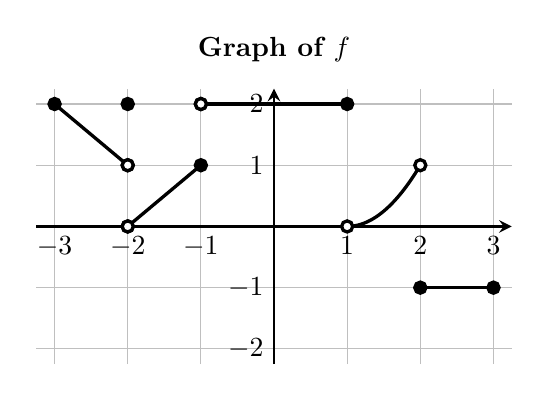
\begin{tikzpicture}
    \begin{axis}[
       	xmin=-3.25, xmax=3.25,
    	ymin=-2.25, ymax=2.25,
    	major tick length={0},
    	xtick={-3,-2,...,3}, ytick={-2,-1,...,2},
    	line width=1pt, title={\textbf{Graph of $f$}},
     	axis lines=center, height=2 in, width=3 in, grid=major,
     	restrict y to domain=-2.25:2.25
    	]
    	\addplot [mark=*, black, smooth, very thick] plot coordinates {(-3,2)(-2,1)};
    	\addplot [mark=*, black, smooth, very thick] plot coordinates {(-2,3)};
    	\addplot [mark=*, black, smooth, very thick] plot coordinates {(-2,0)(-1,1)};
    	\addplot [mark=*, black, smooth, very thick] plot coordinates {(-1,2)(1,2)};
    	\addplot [mark=*, black, smooth, very thick] plot coordinates {(2,-1)(3,-1)};
        \addplot [black, smooth, very thick, samples=100, domain=1:2] {(x-1)^2};
        \addplot [black, only marks, very thick, mark=*, mark options={scale=1, fill=white}]
        coordinates{(1,0) (2,1) (-1,2) (-2,1) (-2,0)};
        \addplot [black, only marks, very thick, mark=*] coordinates{(-2,2)};
    \end{axis}
    \end{tikzpicture}
    %\end{center}
    }
    \end{minipage}}
    
    \newcommand{\ggraff}{
    \begin{minipage}[l][.30\textwidth]{3 in}{
    %\begin{center}
    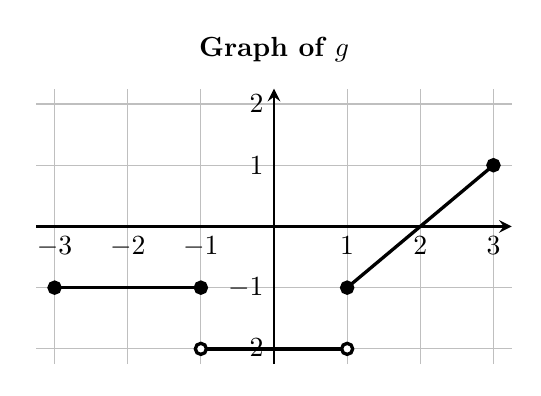
\begin{tikzpicture}
    \begin{axis}[
       	xmin=-3.25, xmax=3.25,
    	ymin=-2.25, ymax=2.25,
    	major tick length={0},
    	xtick={-3,-2,...,3}, ytick={-2,-1,...,2},
    	line width=1pt, title={\textbf{Graph of $g$}},
     	axis lines=center, height=2 in, width=3 in, grid=major,
     	restrict y to domain=-2.25:2.25
    	]
    	\addplot [mark=*, black, smooth, very thick] plot coordinates {(-3,-1)(-1,-1)};
    	\addplot [mark=*, black, smooth, very thick] plot coordinates {(1,-1)(3,1)};
    	\addplot [black, very thick, mark=*, mark options={scale=1, fill=white}] plot coordinates {(-1,-2)(1,-2)};
    \end{axis}
    \end{tikzpicture}
    %\end{center}
    }
    \end{minipage}}
    
    \begin{document}
    
    \begin{center}
        \large \textbf{Homework 2}
    \end{center}
        %\item[\textbf{Week 2}]
                    \begin{enumerate}
                        \item Using the laws of logarithms and properties of summations, show that $$\ln\left(\prod_{k=1}^n \frac{\lambda^{x_k}e^{-\lambda}}{x_k!}\right)=\ln(\lambda)\sum_{k=1}^n x_k -n\lambda - \sum_{k=1}^n \ln(x_k!)$$
                        \item Evaluate each of the following sums.  These same sums will be seen again later in this course in the context of computing the area between a function and the $x$-axis.
                            \begin{enumerate}
                                \item $ \sum_{j=1}^{10} \left(\frac{1}{5}j+4\right)$  (Note that your answer should be a positive numeric value.)
                                \item $ \sum_{j=1}^{8} \frac{1}{2}\left[\left(1+\frac{j}{2} \right)^2 -4\left( 1+ \frac{j}{2}\right) + 5\right]$  (Note that your answer should be a positive numeric value.)
                                \item $ \sum_{j=1}^{n} \frac{4}{n}\left[ \left(\frac{4j}{n}\right)^2 - \frac{4j}{n} + 1 \right]$  (Note that your answer should be an expression in the variable $n$.)
                            \end{enumerate}
                        \item Write the summation as an equivalent summation with the index of summation starting at $k=0$.
                            \begin{enumerate}
                                \item $ \sum_{k=1}^n \frac{n!}{(k-1)!(n-k)!}p^k(1-p)^{n-k}$
                                \item $ \sum_{k=4}^{98} 5\left(\frac{2}{3}\right) ^k$
                            \end{enumerate}
                        \item Evaluate each of the following sums.  Your answer should be an expression in the variable $m$.
                            \begin{enumerate}
                                \item $ \sum_{k=5}^{m} (3k-4)$  (Hint: Consider reindexing to apply the formulas for special sums.)
                                \item $ \sum_{k=2}^{m} (k^3+k^2)$  (Hint: Apply formulas for special sums and then subtract the extra value(s).)
                            \end{enumerate}
                        \item Find the following limits:
                        \begin{enumerate}
                            \item   $ \lim_{x \rightarrow 2^-} \frac{(x^2-4)(x^3-8)}{(x-2)^3}$
                            \item  $ \lim_{h\rightarrow 0} \frac{(x+h)^2-x^2}{h}$
                            \item $ \lim_{x\rightarrow 0} \frac{\left|x\right|}{x}$
                            \item $ \lim_{x\rightarrow 0} \frac{\left|x^2\right|}{x^2}$
                            \item $ \lim_{x \rightarrow 1} \frac{x^2-1}{|x-1|}$ (Hint: Try viewing it as a piecewise function, taking limits from the left and right separately. Graph it using technology to assure you have defined the function correctly.)
                            \item $ \lim_{x \rightarrow 4} \frac{(x+4)(\sqrt{x}-2)}{x^3-64}$
                        \end{enumerate}
                        \item The following limit questions are quite tricky. Be careful! For example, note that the limit laws only apply if all limits exist. Fully justify your work. You may find the correct answer, but for the wrong reasoning.
    
                        \begin{center}
                        \begin{tabular}{l r}
                        \fgraff & \ggraff
                        \end{tabular}
                        \end{center}
                        \begin{enumerate}
                        \item $ \lim_{x\rightarrow -1} (f(x)+g(x))$
                        \item $ \lim_{x\rightarrow -1} \frac{f(x)}{g(x)}$
                        \item $ \lim_{x \rightarrow -2^-} g(f(x))$
                        \item $ \lim_{x \rightarrow -2^+} g(f(x))$
                        \item $ \lim_{x\rightarrow 1^-} f(g(x))$
                        \item $ \lim_{x\rightarrow 2} \frac{f(x)}{g(x)}$
                        \end{enumerate}
                        
                        
    
    
                    \end{enumerate}
    
    
    \end{document}
